
% LaTeX Template for Project Report, Version 2.0
% (Abstracted from a Major Project Report at CSED, NIT Calicut but can be
% modified easily to use for other reports also.)
%
% Released under Creative Commons Attribution license (CC-BY)
% Info: http://creativecommons.org/licenses/by/3.0/
%
% Created by: Kartik Singhal
% BTech CSE Batch of 2009-13
% NIT Calicut
% Contact Info: kartiksinghal@gmail.com
%
% It is advisable to learn the basics of LaTeX before using this template.
% A good resource to start with is http://en.wikibooks.org/wiki/LaTeX/
%
% All template fields are marked with a pair of angular brackets e.g. <title here>
% except for the ones defining citation names in ref.tex.
%
% Empty space after chapter/section/subsection titles can be used to insert text.
%
% Just compile this file using pdflatex after making all required changes.

\documentclass[12pt,a4paper]{report}
\usepackage[pdftex]{graphicx} %for embedding images
\usepackage{url} %for proper url entries
\usepackage[bookmarks, colorlinks=false, pdfborder={0 0 0}, pdftitle={<pdf title here>}, pdfauthor={<author's name here>}, pdfsubject={<subject here>}, pdfkeywords={<keywords here>}]{hyperref} %for creating links in the pdf version and other additional pdf attributes, no effect on the printed document
%\usepackage[final]{pdfpages} %for embedding another pdf, remove if not required

\begin{document}
\renewcommand\bibname{References} %Renames "Bibliography" to "References" on ref page
\pagenumbering{roman} %numbering before main content starts
%include other pages
\begin{titlepage}

\begin{center}

\textup{\huge {\bf IDEA PROPOSAL } \\[0.10in] e-Yantra Ideas Competition 2019-20}\\[0.50in]

% Title

     \huge{\bf Smart waste collection management system} \\[0.80in]
       

% Submitted by
\normalsize Submitted by \\
\begin{table}[h]
\centering
\begin{tabular}{lr}  

  &{\textbf{\normalsize Bharath T U}}\\
    &{\textbf{\normalsize Abhijeet.C}}\\
    &{\textbf{\normalsize Joyal T John}}\\
    &{\textbf{\normalsize Gautham Rajesh}}\\

\end{tabular}
\end{table}

\vspace{.01in}
Under the guidance of\\
{\textbf{\large Arun J S}}\\[0.2in]

\vfill



\end{center}

\end{titlepage}


\pagenumbering{arabic} %reset numbering to normal for the main content

\textup{\huge {\bf Introduction/Motivation: } \\[0.90in] }

\large  {The Inability of the current waste collection system to prompt the households to segregate waste before giving it out to the collectors, forcing the collection workers to separate it manually before treatment making their working conditions unhygienic and wasting their time, and lack of proper communication between the collectors and the household leads inefficient path planning without considering which all household actually have/could give waste at the particular time of pick up wasting fuel and time.}\\[0.3in]

\large  {Our solution is a system which consists of two apps one for the households, another for the collectors which become the communication medium between collectors and households, like allowing the household to get the live location of the collection vehicle, notify the collectors which all households actually have/could give waste at pick-up time. To make this communication more hassle free we introduced a dustbin which is provided to each household this dustbin allows us to trace back to the source of the waste if the waste was not segregated and detect if waste is present in it or not each day and it alerts our system via home Wi-Fi and helps to give an optimized path for the collectors to pick the waste.}\\[0.3in]
\newpage %objective changed to problem definition
\textup{\large {\bf Market Research / Literature Survey: } \\[0.20in] }


\Large  { [1] In India, it is estimated that MSW (Municipal Solid Waste) generated in large cities and towns in India is about 0.1 kg, 0.3 – 0.4 kg and 0.5 kg per capita per day respectively. }\\

\Large  {	In most of the cities in India, the MSW collection, segregation, transportation, processing and disposal are carried by Private collectors or respective municipal corporations }\\[0.003in]
	
\Large {	The collection and transportation section are in of loss because some households do not have/could not give waste at a particular time and as for the segregation part the waste may come mixed but there is no way of tracking them to its source hence not prompting households to segregate waste.}\\[0.003in]
	
\Large {	There are many software-based waste management systems but most of them are targeted at waste collection from a large-scale events or public places, none are targeted for daily household waste collection and they have their own collection workers to collect waste. }\\[0.3in]
\newpage

\textup{\large {\bf Hardware requirements: } \\[0.00001in] }
\begin{enumerate} %Job Description%
	\item{\normalsize {\bf Arduino Nano} would be used in the dustbin to get readings from the sensors and transmit it via Wi-Fi through ESP module }
	\item {\normalsize  {\bf ESP module} will be used to connect the dustbin to the home Wi-Fi}
	\item {\normalsize {\bf Weight Sensor} (just a button which will become closed after a certain amount of waste getting the actual measurement of weight is not required) to sense if there is any waste inside the dustbin or not }
	\item {\normalsize  {\bf RF ID} Reader and chip to track each dustbin}
	\item {\normalsize {\bf Power Adapter} to power the system inside the dustbin \\}
\end{enumerate}
%%%%%%%%%%%%%%%%%%%
%%%%%%%%%%%%%%%%%%%
%%%%%%%%%%%%%%%%%%%
\textup{\large {\bf Software requirements: } \\[0.00001in] }
\begin{enumerate} %Job Description%
	\item{\normalsize {\bf Flutter} for developing the two apps needed}
	\item {\normalsize  {\bf Django} for developing a back-end server for collecting data from the apps and dustbin to run the whole management system}
	\item {\normalsize {\bf	Arduino IDE} for coding the control board used in the dustbin }
	\item {\normalsize  {\bf RF ID} Reader and chip to track each dustbin}
	\item {\normalsize {\bf Power Adapter} to power the system inside the dustbin}
\end{enumerate}
%%%%%%%%%%%%%%%%%%%

\newpage %literature survey included in this


\textbf{\textup{\huge {\bf Implementation: } \\[0.20in] }}

\normalsize { Each day an optimised path will be made by the system with respect to which all household have waste inside their dustbin(this info is taken via the dustbins internal system or the household user can manually override and prompt for a pick up) and the path is given for each collection vehicle to pick up waste and a notification is sent to each household to ask if they could give the waste at the specific time of the collections vehicles arrival, they could check the live location of the collection vehicle via the app and give their response. The path will be optimised again with respect to each household’s response. If the household didn’t or couldn’t give waste even after responding they could they will be fined.}\\[0.1in] 
\normalsize { 	When the collection vehicle comes near a specific household they could slide the dustbin out of a dock which houses the sensing and Wi-Fi system and give the dustbin to the collection worker, the worker would give a clean dustbin which was taken from the collection vehicle and take the full dustbin to replace it in the vehicle. The new clean dustbin can be slid back into the dock and the dock will read the RF-ID chip which is every bin is equipped with and register the serial number of the bin, current date and the household where it has been placed into the systems server via home Wi-Fi. 
	. }\\[0.1in]

	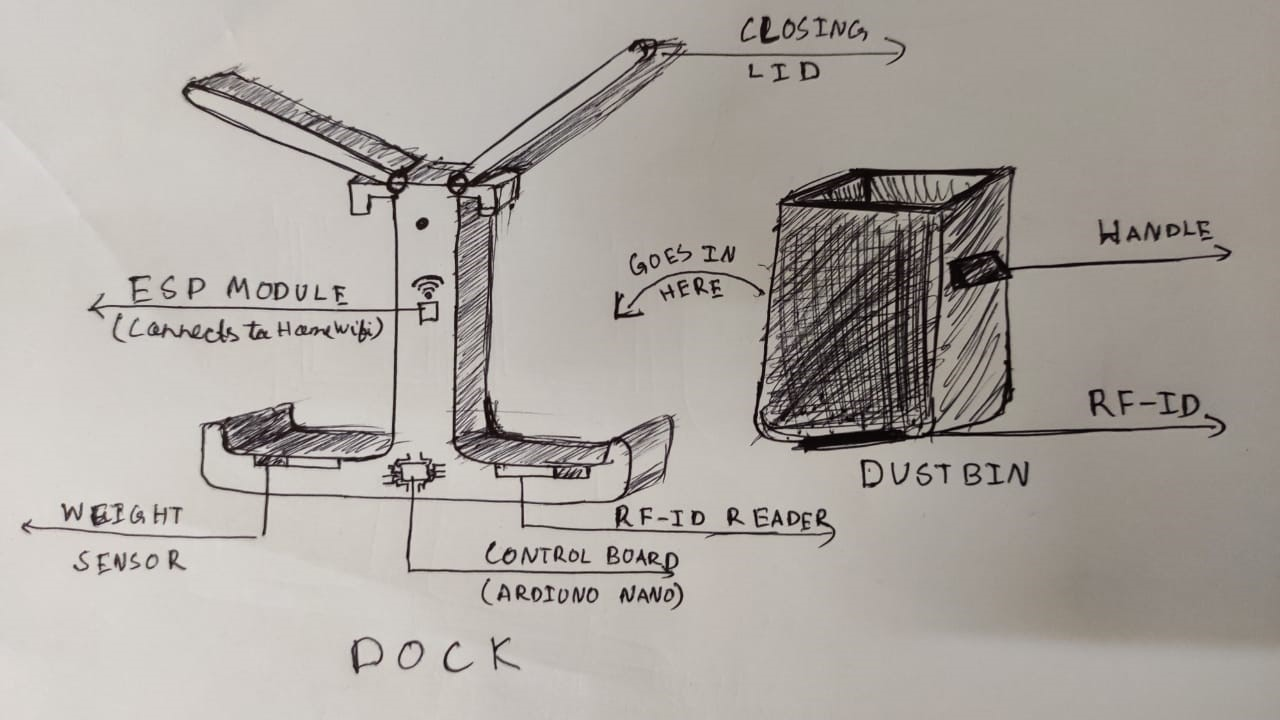
\includegraphics[width=\linewidth]{pic1.jpg}
\\[0.3in]
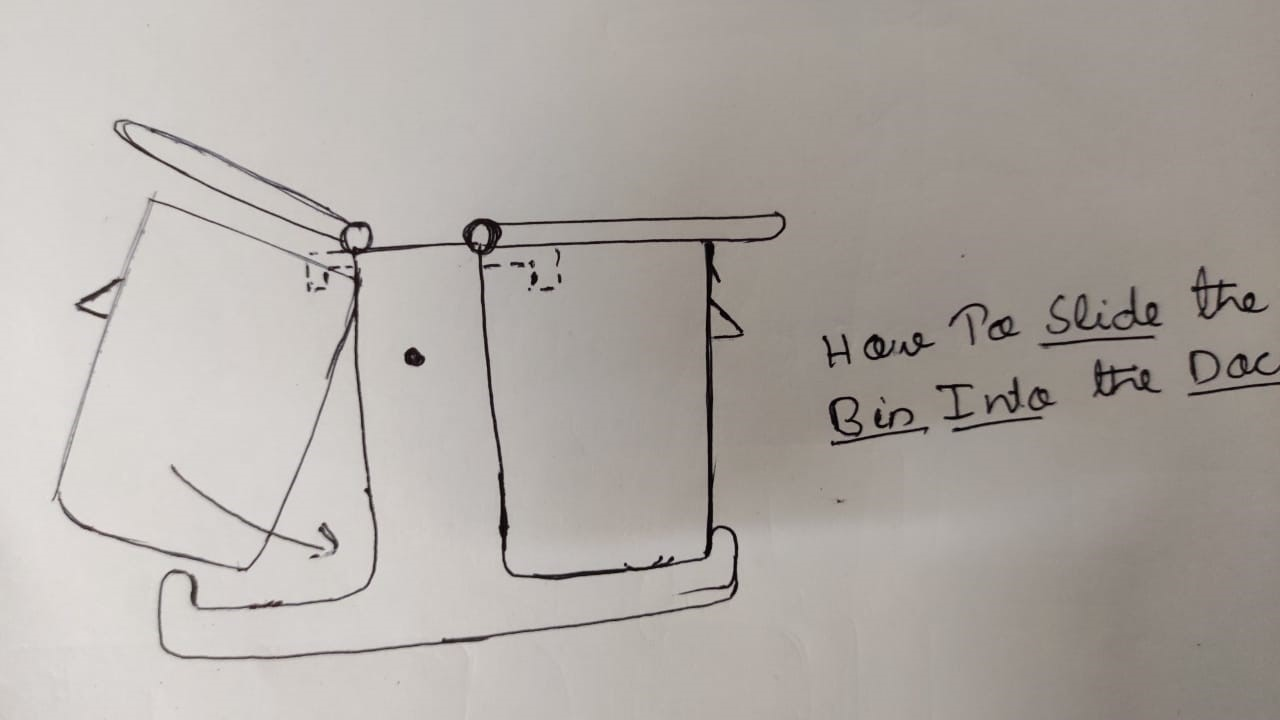
\includegraphics[width=\linewidth]{pic2.jpg}\\[0.3in]

\normalsize {After the collection vehicle has done collecting it will go to the waste treatment plant and clear each of the bins if one of the bins are found to have mixed waste the source of the waste is found by tracking its serial number of the RF ID via the server’s database and that household would be fined. After all the dustbins are cleared, they are cleaned by pressurised water and circulated back. As each dock will register each time the dustbin is changed, we could count the number of days a specific house used the collection service and bill them accordingly so and each house hold could pay through our system and the collection workers will get the money via our system (like uber).}\\[0.01in]

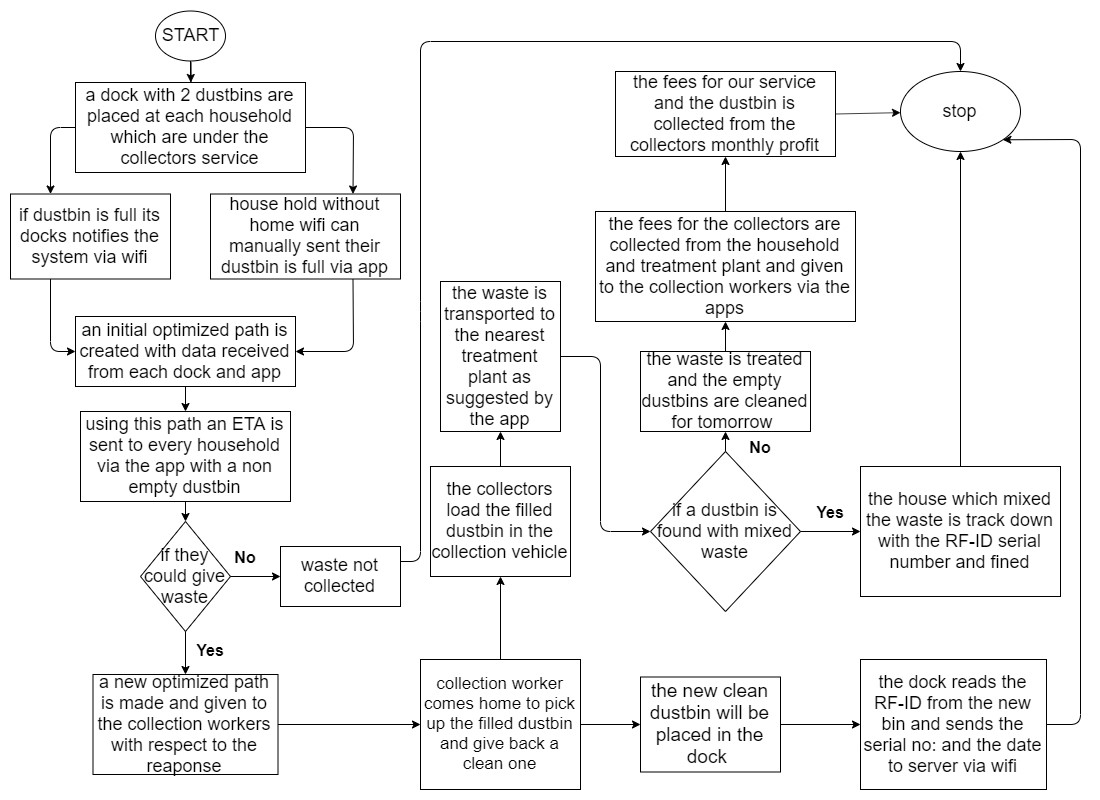
\includegraphics[width=\linewidth]{flow.jpg}\\[0.3in]


\normalsize {The main way we will get the money for our services that is the two apps, the management system and the dustbins are by taking a fraction of the monthly profit of the collection workers and the interest of the caution deposit taken for each dustbin. The dustbin and the dock together is estimated to cost around 1200Rs per household and we will take a caution deposit of 600Rs from the households and give install it in their house, and 10 percentage of the monthly profit (excluding the fines collected from household for malpractice) of the collection workers will be taken by us. Although the dustbins are manufactured by us and given out for free of cost like a net router provided by a ISP but will still be owned by us. As for the cleaning of the dustbins must be done by the collection workers we will provide them the equipment for seemingly free of cost.
}\\[0.1in]


	
\newpage

\textup{\huge {\bf Prototyping Cost: } \\[0.01in] }

\textup{\large {\bf Hardware: } \\[0.00001in] }
\begin{enumerate} %Job Description%
	\item{\normalsize {\bf Arduino Nano} : Rs 250}
	\item {\normalsize  {\bf ESP module} : Rs 150 }
	\item {\normalsize  {\bf RF ID } :  Rs 135x2 }
	\item {\normalsize  {\bf Sliding Dustbin } :  Rs1000  }
	\item {\normalsize {\bf Power Adapter} : Rs 200 \\}
\end{enumerate}
\textup{\large {\bf Software: } \\[0.00001in] }
\begin{enumerate} %Job Description%
	\item{\normalsize {\bf Servera and Domain} : Rs 800}

\end{enumerate}
\newpage

\textup{\huge {\bf Feasibility: } \\[0.01in] }


\large {The current daily household waste management system has various limitation 2 of the major one being waste segregation and the other is waste collection.
	In order to efficiently collect daily waste from households and manage them we came up with a solution that is to connect the households and the collectors via apps and share data between them through the dustbins at each household.\\[0.01in] 
	\large {
	The current problems of waste segregation and transportation are solved by our solution. This allows the collection workers to have a more hygienic working environment and save fuel by not going to every single house every day.
	.}\\[0.1in]

\textup{\huge {\bf References: } \\[0.01in] }

\large { [1]Municipal Solid waste (2019). On use of municipal solid waste in India
}\\[0.1in]
\large{LINK: \url{http://www.eai.in/ref/ae/wte/typ/clas/msw.html}[onine]}

\end{document}
